% This is a LaTeX thesis template for Monash University.
% to be used with Rmarkdown
% This template was produced by Rob Hyndman
% Version: 6 September 2016

\documentclass{monashthesis}

%%%%%%%%%%%%%%%%%%%%%%%%%%%%%%%%%%%%%%%%%%%%%%%%%%%%%%%%%%%%%%%
% Add any LaTeX packages and other preamble here if required
%%%%%%%%%%%%%%%%%%%%%%%%%%%%%%%%%%%%%%%%%%%%%%%%%%%%%%%%%%%%%%%

\author{Zhixiang Yang}
\title{Disaggregated Sectoral Employment Dynamics in Australia}
\studentid{30306396}
\def\degreetitle{Bachelor of Commerce (Honours)}
% Add subject and keywords below
\hypersetup{
     %pdfsubject={The Subject},
     %pdfkeywords={Some Keywords},
     pdfauthor={Zhixiang Yang},
     pdftitle={Disaggregated Sectoral Employment Dynamics in Australia},
     pdfproducer={Bookdown with LaTeX}
}


\bibliography{thesisrefs}

\begin{document}

\pagenumbering{roman}

\titlepage

{\setstretch{1.2}\sf\tighttoc\doublespacing}

\clearpage\pagenumbering{arabic}\setcounter{page}{0}

\graphicspath{ {/Users/elvisyang/Desktop/hon_proj/Disaggregated_Employment/Honours_thesis/figure} }

\hypertarget{acknowledgement}{%
\chapter*{Acknowledgement}\label{acknowledgement}}
\addcontentsline{toc}{chapter}{Acknowledgement}

I would like to express gratitude to my supervisor Professor Farshid Vahid and my coordinatior Professor Heather Anderson for their selfless support and devoted care along the way.

\hypertarget{declaration}{%
\chapter*{Declaration}\label{declaration}}
\addcontentsline{toc}{chapter}{Declaration}

I declare that this thesis contains no material which has been submitted in any form for the award of any other degree or diploma in any university or equivalent institution, and that, to the best of my knowledge and belief, this thesis contains no material previously published or written by another person, except where due reference is made in the text of the thesis.

\hypertarget{abstract}{%
\chapter*{Abstract}\label{abstract}}
\addcontentsline{toc}{chapter}{Abstract}

We develop a multivariate time series model of employment in Australia at a disaggregated level with 87 sectors in total. We use this model to determine the long run employment spillovers to the total employment at this level. Our findings is that \ldots{} Moreover, we provide an interactive shiny app that will give an intuitive visualization of these changes. At the stage of recovering from COVID-19, it will provide more useful information for policymakers on recovering total employment rate more effectively.

\hypertarget{the-australian-covid-19-pandemic-background}{%
\chapter{The Australian COVID-19 Pandemic Background}\label{the-australian-covid-19-pandemic-background}}

The COVID-19 pandemic has had a massive effect on economies around the world. Across different countries, millions of workers were furloughed or even lost their jobs as businesses struggled to survive \autocite{ny2020}. The same situation happened in Australia, due to more restrictions, many businesses closed their doors, while employees were working with less hours or being dismissed by companies. As a result of the continuous ``lockdown'' periods in 2020, estimates made by the Australian Bureau of Statistics \autocite{ABS2021} concluded that 72\% of businesses generated less revenue and the underemployment rate hit a historical high of 13.8\% by the end of April, 2020, only one month after the COVID-19 outbreak.

Our research is motivated by the lack of quantitative research on the employment of two-digit disaggregated industry sectors in Australia, as many studies have focused on the aggregated employment rate. A general problem of aggregated research is the loss of hierarchical information, which may result in a biased conclusion or ``an illusion of employment prosperity''. Thus, a quantitative analysis of the sectoral employment will ameliorate this problem, giving us a better scope to evaluate the impacts of COVID-19 in Australia.

\hypertarget{research-aim-and-questions}{%
\section{Research Aim and questions}\label{research-aim-and-questions}}

This research will extend \textcite{anderson2020} by using data on 87 two-digit industry sectors instead of 19 sectors that they used. I will develop a model for the two-digit sectors to evaluate the long run effect and the COVID-19 post-impacts. I will also provide a counterfactual analysis based on the assumption ``if there is no pandemic''. The two-digit sectoral data will provide us with more information, which will assist in getting a better understanding of employment dynamics in Australia.

The overall research aim is to provide estimates of two-digit sectoral employment based on historical data. Specifically, my goals are:

\begin{enumerate}
\def\labelenumi{\arabic{enumi}.}
\item
  To construct a time series model of employment in 87 two-digit sectors of the Australian economy.
\item
  To use this model to conduct a counterfactual analysis.
\item
  To use this model to determine which two-digit sectors have the highest impact (or positive spillover) on employment growth in the long run.
\end{enumerate}

\hypertarget{thesis-structure}{%
\section{Thesis Structure}\label{thesis-structure}}

This thesis focus on analyzing Australian Employment at a disaggregated level, then estimate the long run effects of the COVID-19 to sectoral employment rate in Australia. The remainder of the thesis is structured as follows. In chapter 2, we review the existing literature in the relevant fields. In chapter 3, we will provide exploratory data analysis and data resources.

\hypertarget{review-of-literature}{%
\chapter{Review of literature}\label{review-of-literature}}

Our review of literature mainly focuses on two areas:

\begin{enumerate}
\def\labelenumi{\arabic{enumi}.}
\item
  The COVID-19 sectoral impacts and modelling of the economy.
\item
  Modelling of large numbers of time series.
\end{enumerate}

\hypertarget{sectoral-impact-of-covid-19.}{%
\section{Sectoral Impact of COVID-19.}\label{sectoral-impact-of-covid-19.}}

Most existing studies have focused on the evaluation of the impacts of COVID-19 on broad sectors of large economies such as the US and Europe. \textcite{ludvigson2020covid} developed a disaster series to translate the macroeconomic impact of costly and deadly disasters in recent US history and model them as sectoral shocks to predict COVID-19. They concluded that the shock would lead to a cumulative loss of 20\% in industrial production, 39\% in public services and also reduce the US GDP by 12.75 per cent at the end of 2020. \textcite{gregory2020pandemic} conducted simulations under different scenarios via a search theoretic model using US data and found the recovery in the US is L-shaped, with employment remaining lower than pre-covid for a long period. They also extended their studies at a disaggregated level of 20 sectors, showing that ``arts and entertainment'' and ``accommodation and food services'' sectors would have the biggest shock during the pandemic.

In Australia, \textcite{anderson2020} developed a multivariate time series model for 19 main sectors in Australia (as a small open economy) using a Bayesian VARX model. Their research concluded that ``Manufacturing'' and ``Construction'' have the highest positive spillovers for the aggregate economy. Meanwhile, they also applied a ``conditional forecasting'' method proposed by \textcite{waggoner1999} to simulate different scenarios for the pandemic in Australia. However, their research does not use a finely disaggregated level in Australia (two-digit subsectors of main sectors), which can be extremely useful in macroeconomic analysis.

\hypertarget{modelling}{%
\section{Modelling}\label{modelling}}

\hypertarget{baysian-var}{%
\subsection{Baysian VAR}\label{baysian-var}}

The Bayesian Vector Autoregression model (BVAR) is commonly used in the literature for multivariate data \autocites[e.g.][]{anderson2020,litterman1986,banbura2010large}. The BVAR model is attractive because it allows us to estimate a large number of parameters, when the sample size is not large, in a statistically coherent way.\autocite{litterman1986,wozniak2016bayesian}.

In order to utilize the Bayesian VAR estimators \textcite{litterman1979} proposed the Minnesota Prior, which decreases the weight of the lagged variable with the lag length. The prior mean on the first own lag is set to unity and the rest are set to zero so that (a) the most recent lag should provide more information than distant lags; and (b) own lags should explain more than the lags of other variables.

\hypertarget{improvement-of-bvar}{%
\subsection{Improvement of BVAR}\label{improvement-of-bvar}}

The literature suggests that a significant improvement can be made in large BVAR dynamic models by imposing a stronger shrinkage parameter \autocite{banbura2010large,litterman1986}. \textcite{robertson1999vector} and \textcite{kadiyala1997} proposed a Normal-inverse-Wishart prior which retains the principal of Minnesota prior. Meanwhile, \textcite{banbura2010large} suggested an easier way to apply the Minnesota prior via adding dummy observations into the BVAR system.

\hypertarget{data-collection-and-exploratory-analysis}{%
\chapter{Data collection and exploratory analysis}\label{data-collection-and-exploratory-analysis}}

\hypertarget{data-introduction}{%
\section{Data Introduction}\label{data-introduction}}

Our data source is the ABS Employment by industry subdivision of main job \autocite{ABS2022}, which records employment (measured in \(thousands\)) by the ANZSIC industry sub-division of their main jobs from \(1984:Q4\) to \(2021:Q4\). Our data structure is provided via Figure \ref{fig:anzsic}.

Although seasonally adjusted data is available in \autocite{ABS2022}, I will work with the original data to capture any possible changes in seasonal patterns. I will apply a seasonal difference the logarithm of the original series in order to make them stationary and eliminate seasonality, which will make it easier to conduct further steps.

\hypertarget{preliminary-exploratory-data-analysis}{%
\section{Preliminary Exploratory Data Analysis}\label{preliminary-exploratory-data-analysis}}

\newpage

Figure \ref{fig:19} illustrates the changes in the raw data for 19 main sectors in Australia during the pandemic. Due to the closedown of businesses and travel bans on 2020:Q2, we can observe that the total employment number dropped substantially (from around 13,200,000 to 12,200,000 on \(2020:Q2\)). Most industries behaved similarly with significant changes shown in Figure \ref{fig:19} . Comparing with the previous data of these industries,'' Accommodation \& Food'', ``Media \& telecom'' and Administrative industries have experienced a severe loss of employment and have not fully recovered to the pre-covid level. However, some industries like ``Financial'' and ``Electricity \& Gas'' showed a continuously increasing trend as before.

Nevertheless, there is a drawback of considering the 19 board sectors only; because the two-digit subsectoral dynamics of these sectors may not be homogeneous with their aggregated sectoral changes. For example, when observing the aggregated performance of the ``Manufacturing'' and ``Mining'' sectors from the 19 sectoral level (see Figure \ref{fig:a19}), we may believe that their corresponding subsectors should illustrate the same pattern. However, the reality is that while there is a decreasing trend in the ``Manufacturing'' sector or an increasing trend in the ``Mining'' sector, some of their two-digit subsectors are performed differently (see Figure \ref{fig:a87}). This means that not all two-digit subsectors follow the same pattern with the aggregated sectoral level.

Table \ref{tab:comp} shows the top five and bottom five two-digit subsectors in terms of their employment growth during the pandemic. From \ref{tab:comp} we can conclude that the ``Forestry and Logging'' experienced a severe shock after the lockdown happened on 2020:Q2, followed by ``Private Households Employing Staff'' and ``Library and Other Information Services''. Figure \ref{fig:87} demonstrates the performance of each industry at a more disaggregated two-digit subsectoral level, we can observe that many two-digit subsectors have also shown huge decreases in employment in 2020:Q2.

\hypertarget{methdology}{%
\chapter{Methdology}\label{methdology}}

\hypertarget{proposed-model}{%
\section{Proposed Model}\label{proposed-model}}

I plan to use a Bayesian VARX model based on a method proposed by \textcite{anderson2020}. In the model, each sector is affected by the lags of sectoral growth and a lag of the total employment growth. The lag of aggregate employment growth acts as an economy-wide factor which will affect each sector.

Under the assumption that the structure of the Australian economy will not change during COVID-19, we suggest the BVAR model as

\[
\begin{aligned}
\textbf{y}_t=\textbf{c}+\textbf{A}_1 \textbf{y}_{t-1}+\textbf{A}_2\textbf{y}_{t-2}+\textbf{A}_3\textbf{y}_{t-3}+\textbf{A}_4\textbf{y}_{t-4}+\bf{\Gamma}\textbf{x}_{t-1}+\bf{u}_t
\end{aligned}
\]

where \(\bf{y}_t\) is an \(87\times1\) vector of two-digit subsectoral employment growth rate at time \(t\) and \(\bf{x}_{t-1}\) is the \(4\times1\) vector of 4 lags of the growth rate of aggregate employment (this vector of variables are predetermined at time \(t\)), \textbf{c} is a vector of constants, \(\bf{A}_{1,2,3,4}\) are \(87\times87\) parameter matrices. \(\bf{\Gamma}\) is a \(87\times4\) matrix and \(\bf{u}_t\) is a vector of reduced form errors with the mean equals to zero and independent variance \(\bf{u}_t \sim (0,\bf{\Sigma})\). (see Appendix)

\hypertarget{prior-and-shrinkage}{%
\section{Prior and shrinkage}\label{prior-and-shrinkage}}

Bayesian VAR helps to overcome the curse of high dimensionality via the imposition of prior beliefs on the parameters \autocite{banbura2010large}. I will estimate the VARX using Bayesian methods by specifying a Minnesota prior \autocites[e.g.][]{anderson2020,litterman1986,robertson1999vector}. In order to set up the Minnesota prior in our BVAR model, \textcite{banbura2010large} suggests a Minnesota-type prior that applies shrinkage to the VAR slope coefficients as follows:

\[
\begin{aligned}\label{eq:1}
&E[a_{j}^{jk}] = E[\gamma_{i}^j]=0\\
\\
&Var[a_j^{jk}]= 
\begin{cases}
\frac{\lambda^2}{i^2},&j=k\\
\frac{\lambda^2}{i^2}\frac{\sigma^2_{j}}{\sigma^2_k},& otherwise
\end{cases}\\
\\
&Var[\gamma_i^{j}]=\frac{\lambda^2}{i^2}\frac{\sigma^2_{j}}{\sigma^2_e}
\end{aligned}
\]
where the degree of shrinkage is governed by \(\lambda\), \(\frac{1}{i^2}\) to down-weight more distant lags and the \(\frac{\sigma_j^2}{\sigma_k^2}\) adjusts for different scale of the data. \(\sigma^2_e\) is the variance after fitting an AR model on total employment growth.

\textcite{banbura2010large} also suggested that a natural conjugate Normal-Inverse-Wishart which retains the principle of Minnesota prior will help in adding Minnesota prior to the Bayesian VAR system. Its posterior moments can be calculated either analytically or through adding the dummy observations. I will use dummy observations to estimate the BVAR \autocites[e.g.][]{banbura2010large,anderson2020,wozniak2016bayesian}. More details are provided in the Appendix.

\hypertarget{sectoral-employment-multiplier-analysis}{%
\section{Sectoral Employment Multiplier Analysis}\label{sectoral-employment-multiplier-analysis}}

I will also conduct a two-digit subsectoral employment multiplier analysis based on the estimated BVAR model and the 87 two-digit subsectoral data.

At each time period, we have :

\[
GR_T=\sum_{j=1}^{87} w_j\times {GR}_j
\]

where \(w_j\) is the share of employment of two-digit subsector \(j\) in the total employment, \(GR_T\) is the growth rate in total employment and \(GR_j\) is the growth rate in employment of two-digit subsector \(j\).

Due to the interconnection of macroeconomic two-digit subsectors, when a two-digit subsector \(j\) has an increase in employment, in the long run, it may have spillover effect onto other two-digit subsectors, especially those that have high connections with the two-digit subsector \(j\) (\textcite{anderson2020}).

If this long-run effect is larger than the immediate effect, then this two-digit subsector will have positive spillover effect on total employment, and \emph{vice versa}. I will use the interconnection of BVAR parameters to estimate two-digit subsectors which have strong positive spillovers for the total employment. Then, if the government makes policies to stimulate these two-digit subsectors, the total employment will recover more effectively.

\newpage

\appendix

\hypertarget{additional-stuff}{%
\chapter{Additional stuff}\label{additional-stuff}}

You might put some computer output here, or maybe additional tables.

Note that \texttt{\textbackslash{}appendix} must appear before your first appendix. But other appendices can just start like any other chapter.

\graphicspath{ {/Users/elvisyang/Desktop/hon_proj/Disaggregated_Employment/Honours_thesis/figures} }

\begin{figure}[t]
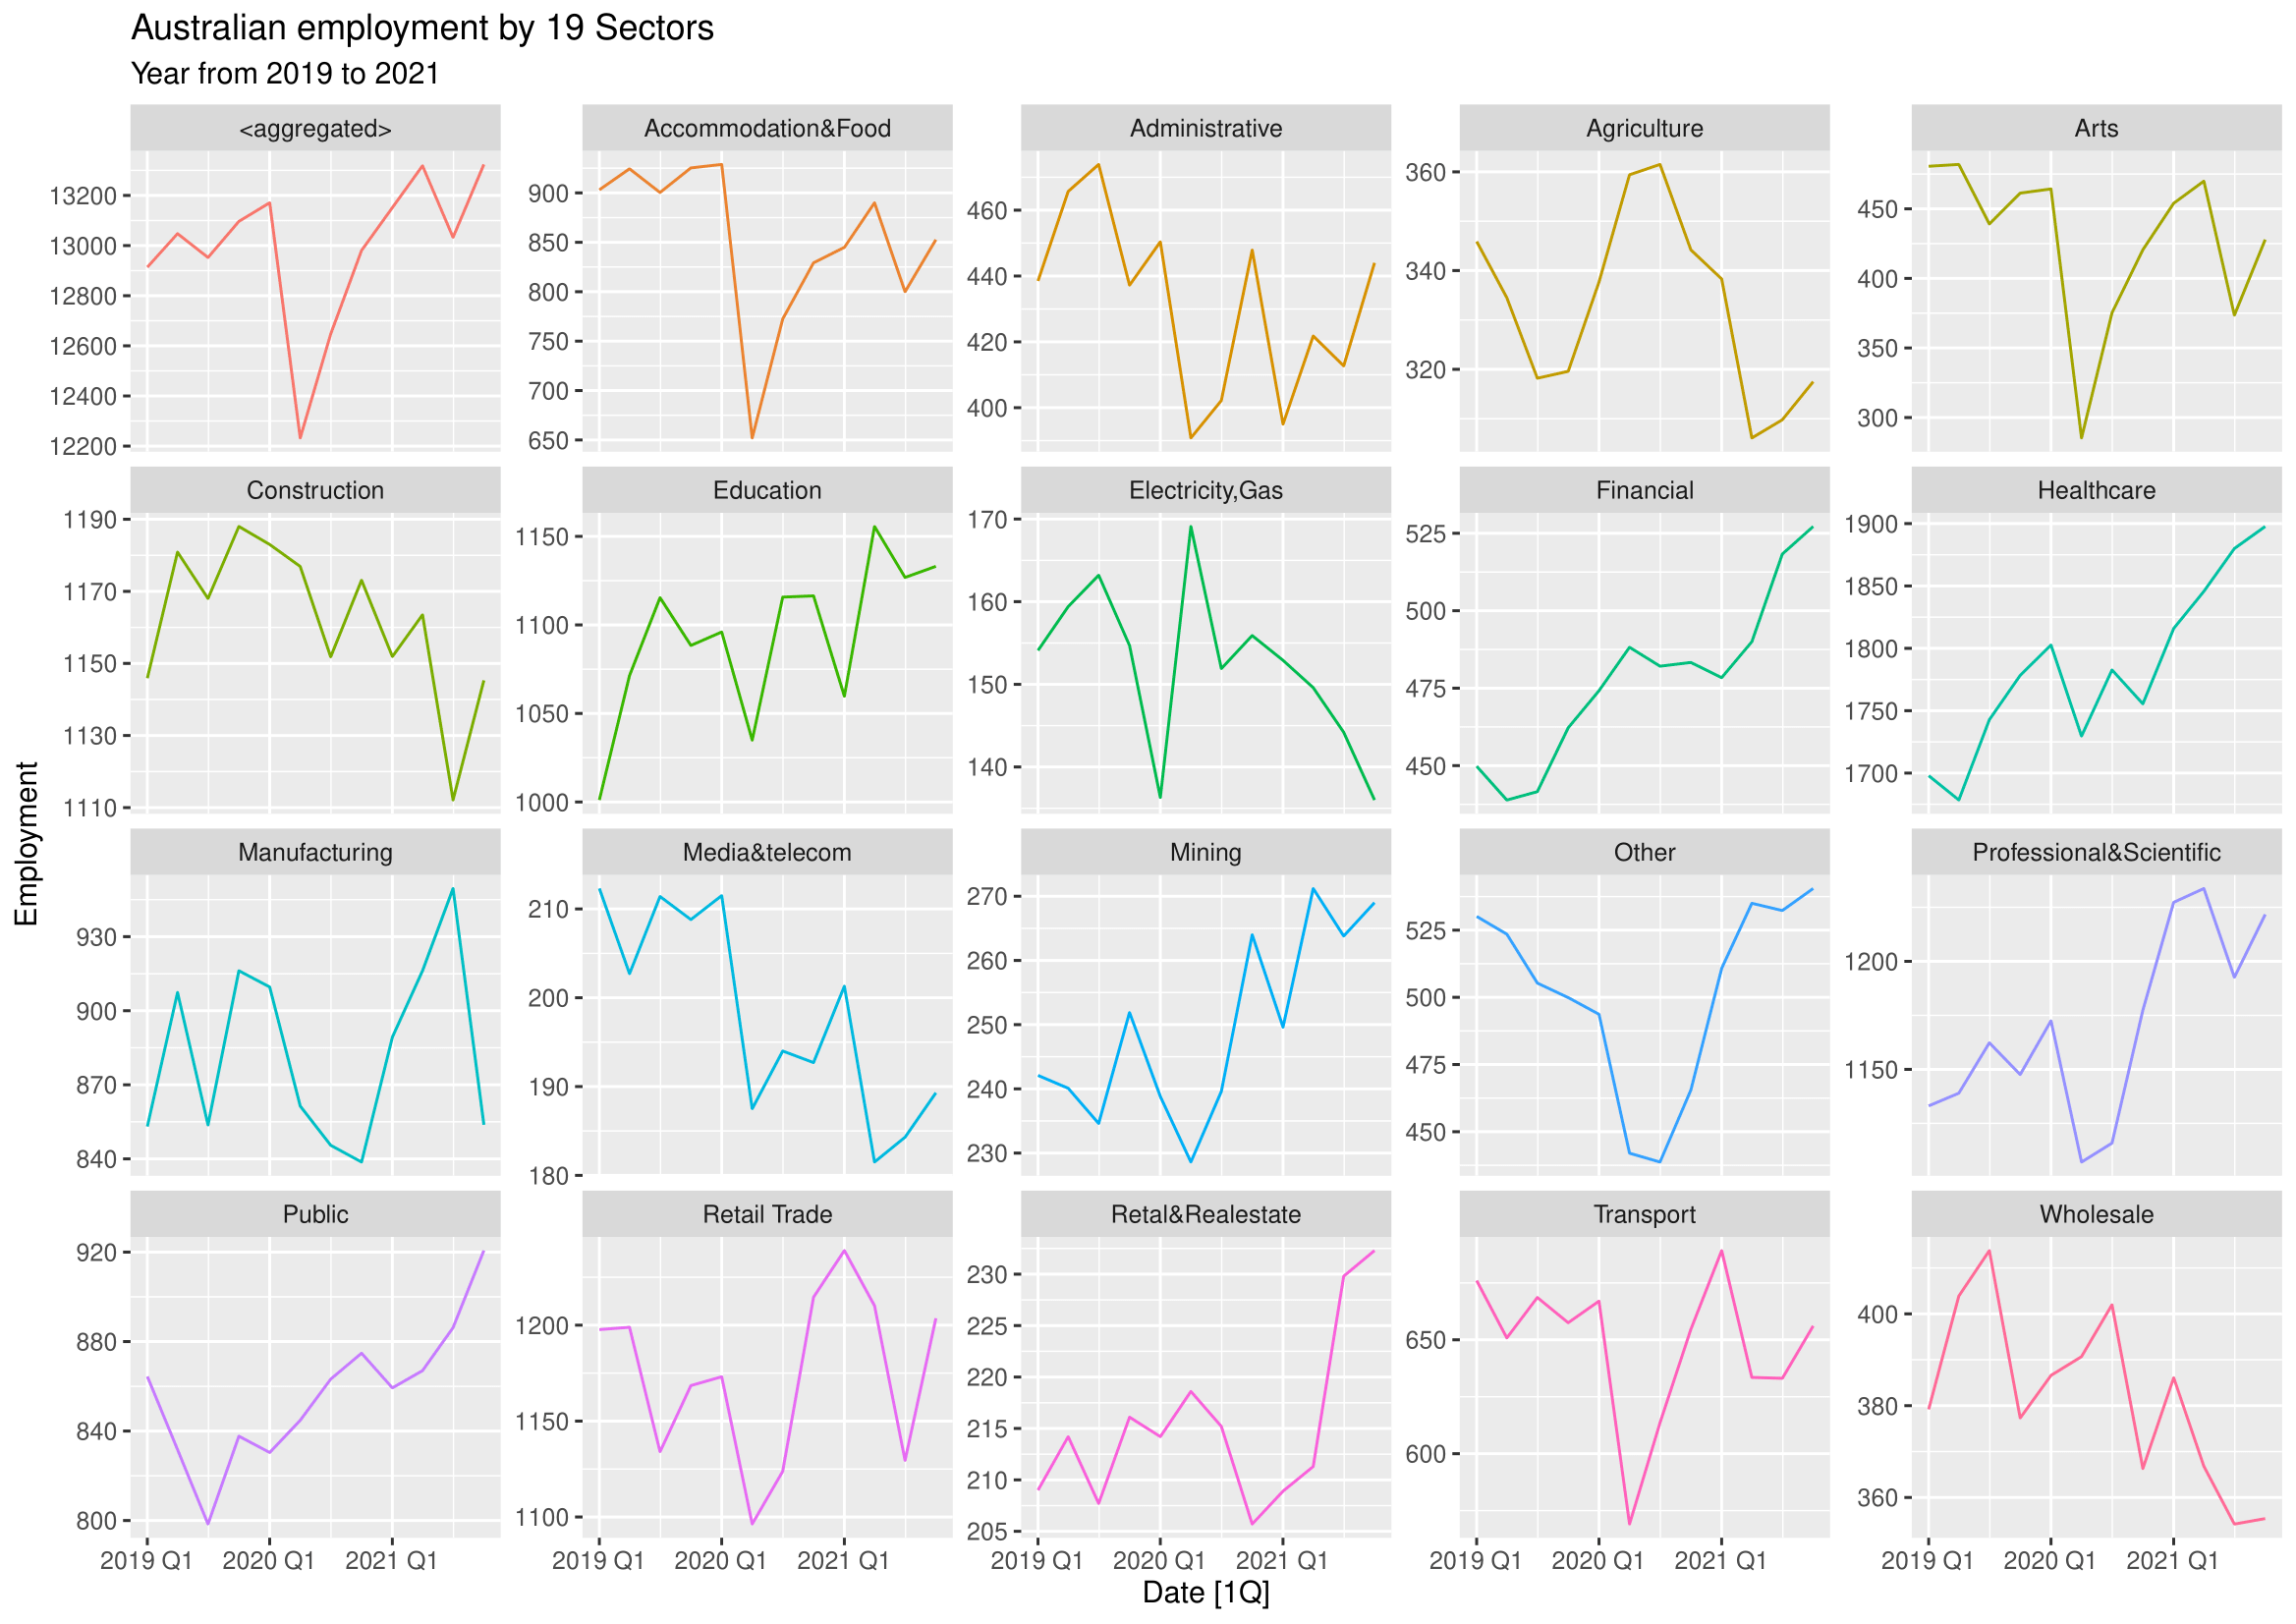
\includegraphics[scale=0.6]{free_19}
\centering
\caption{Employment('000) of 19 sectors in Australia from 2019:Q1 to 2021:Q4}
\label{fig:19}
\end{figure}

\begin{figure}[t]
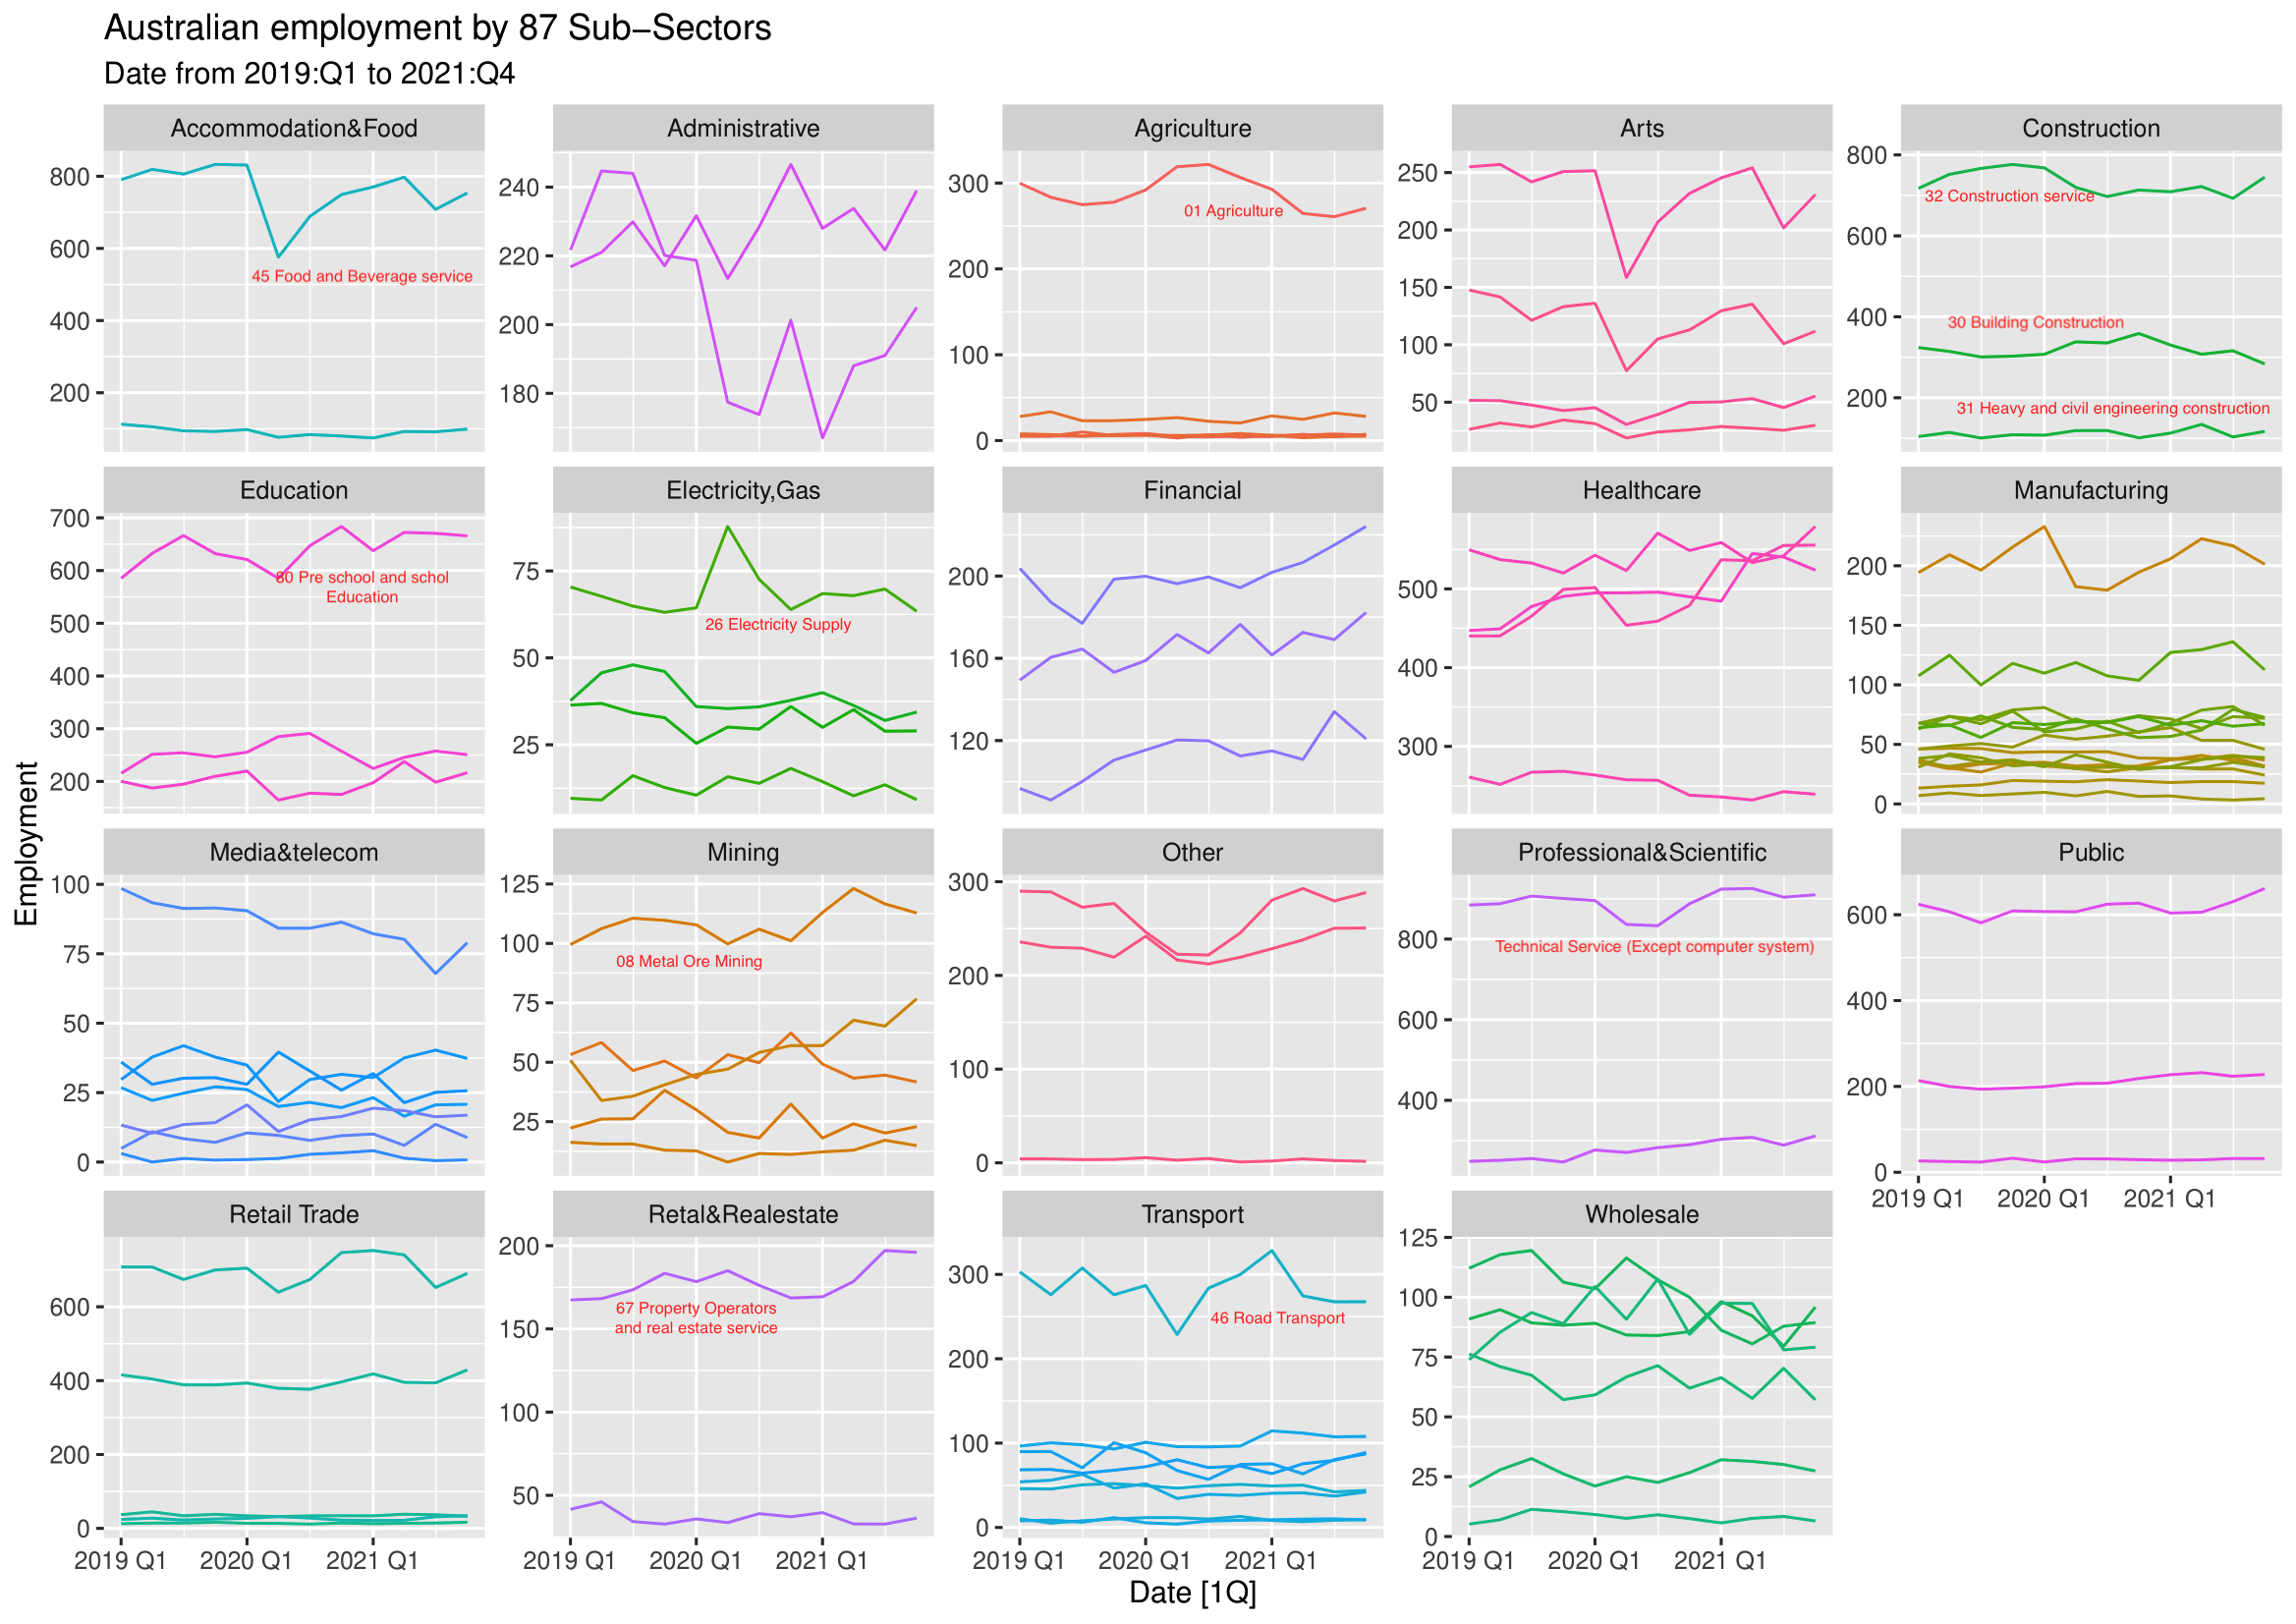
\includegraphics[scale=0.5]{free_87}
\centering
\caption{Employment('000) of 87 two-digit subsectors in Australia from 2019:Q1 to 2021:Q4}
\label{fig:87}
\end{figure}

\begin{figure}[t]
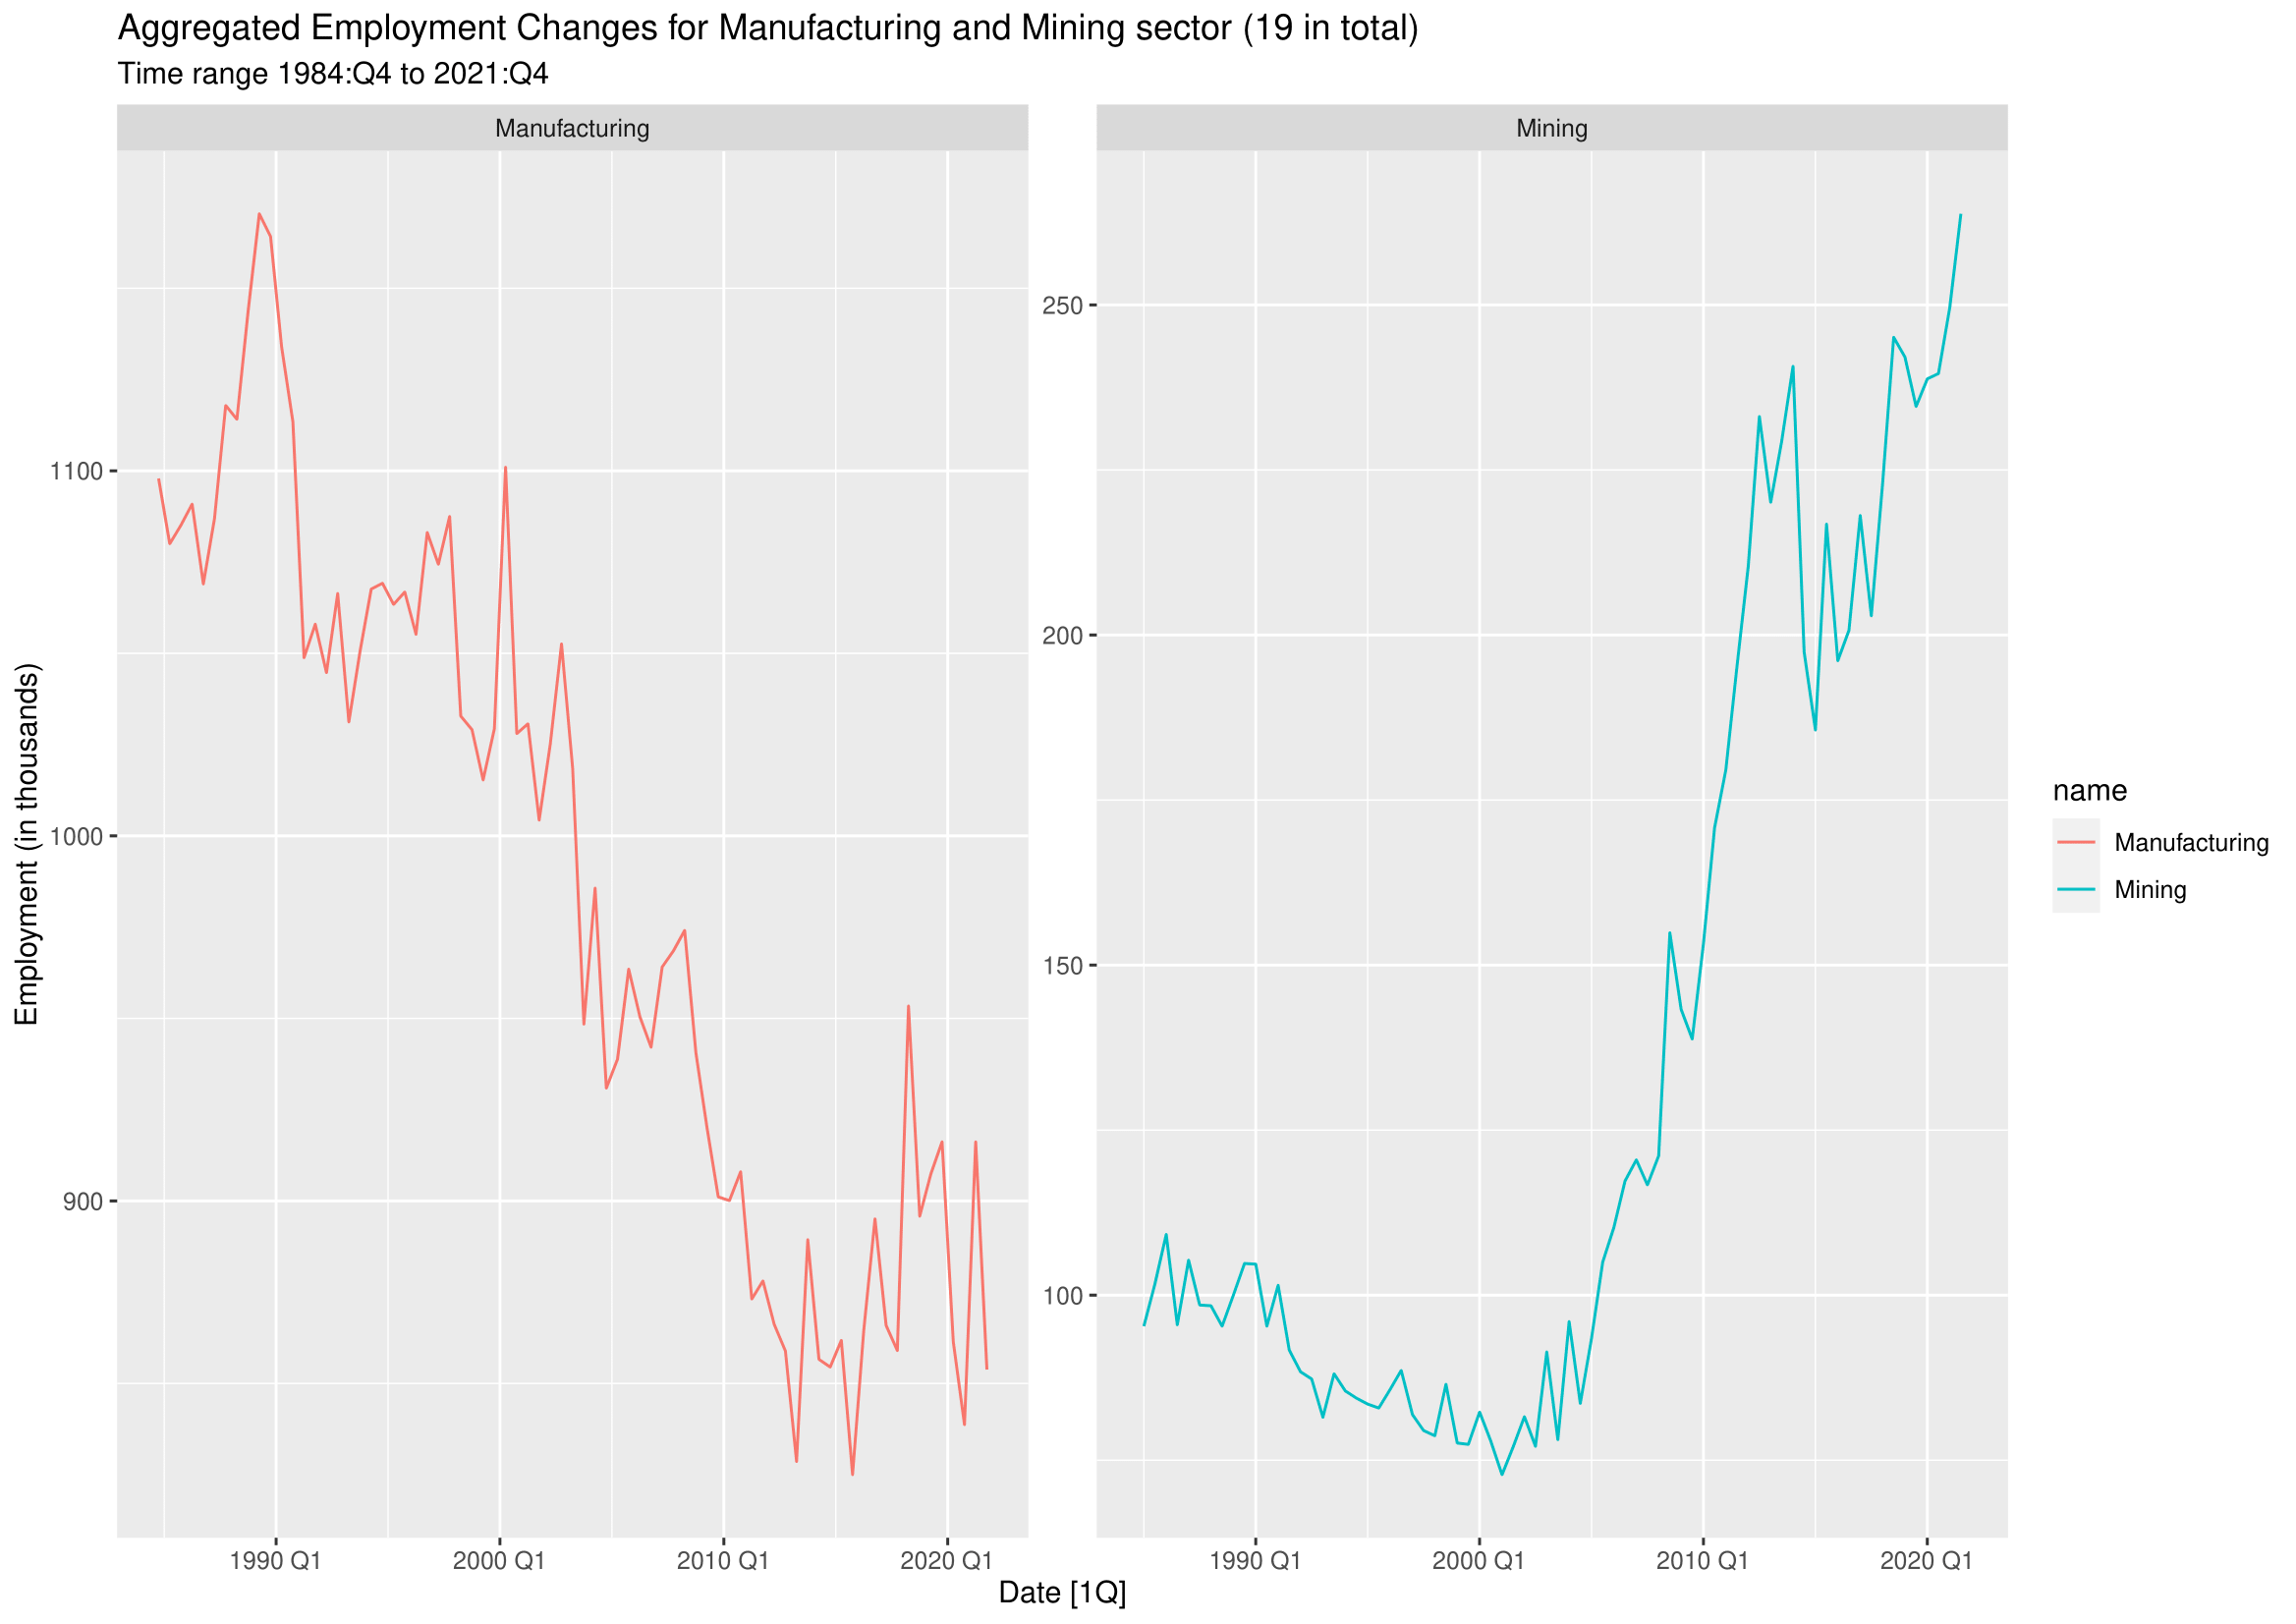
\includegraphics[scale=0.5]{agg_19}
\centering
\caption{Aggregated Employment(in thousands) for Manufacturing and Mining sector in Australia from 1984:Q4 to 2021:Q4}
\label{fig:a19}
\end{figure}

\begin{figure}[t]
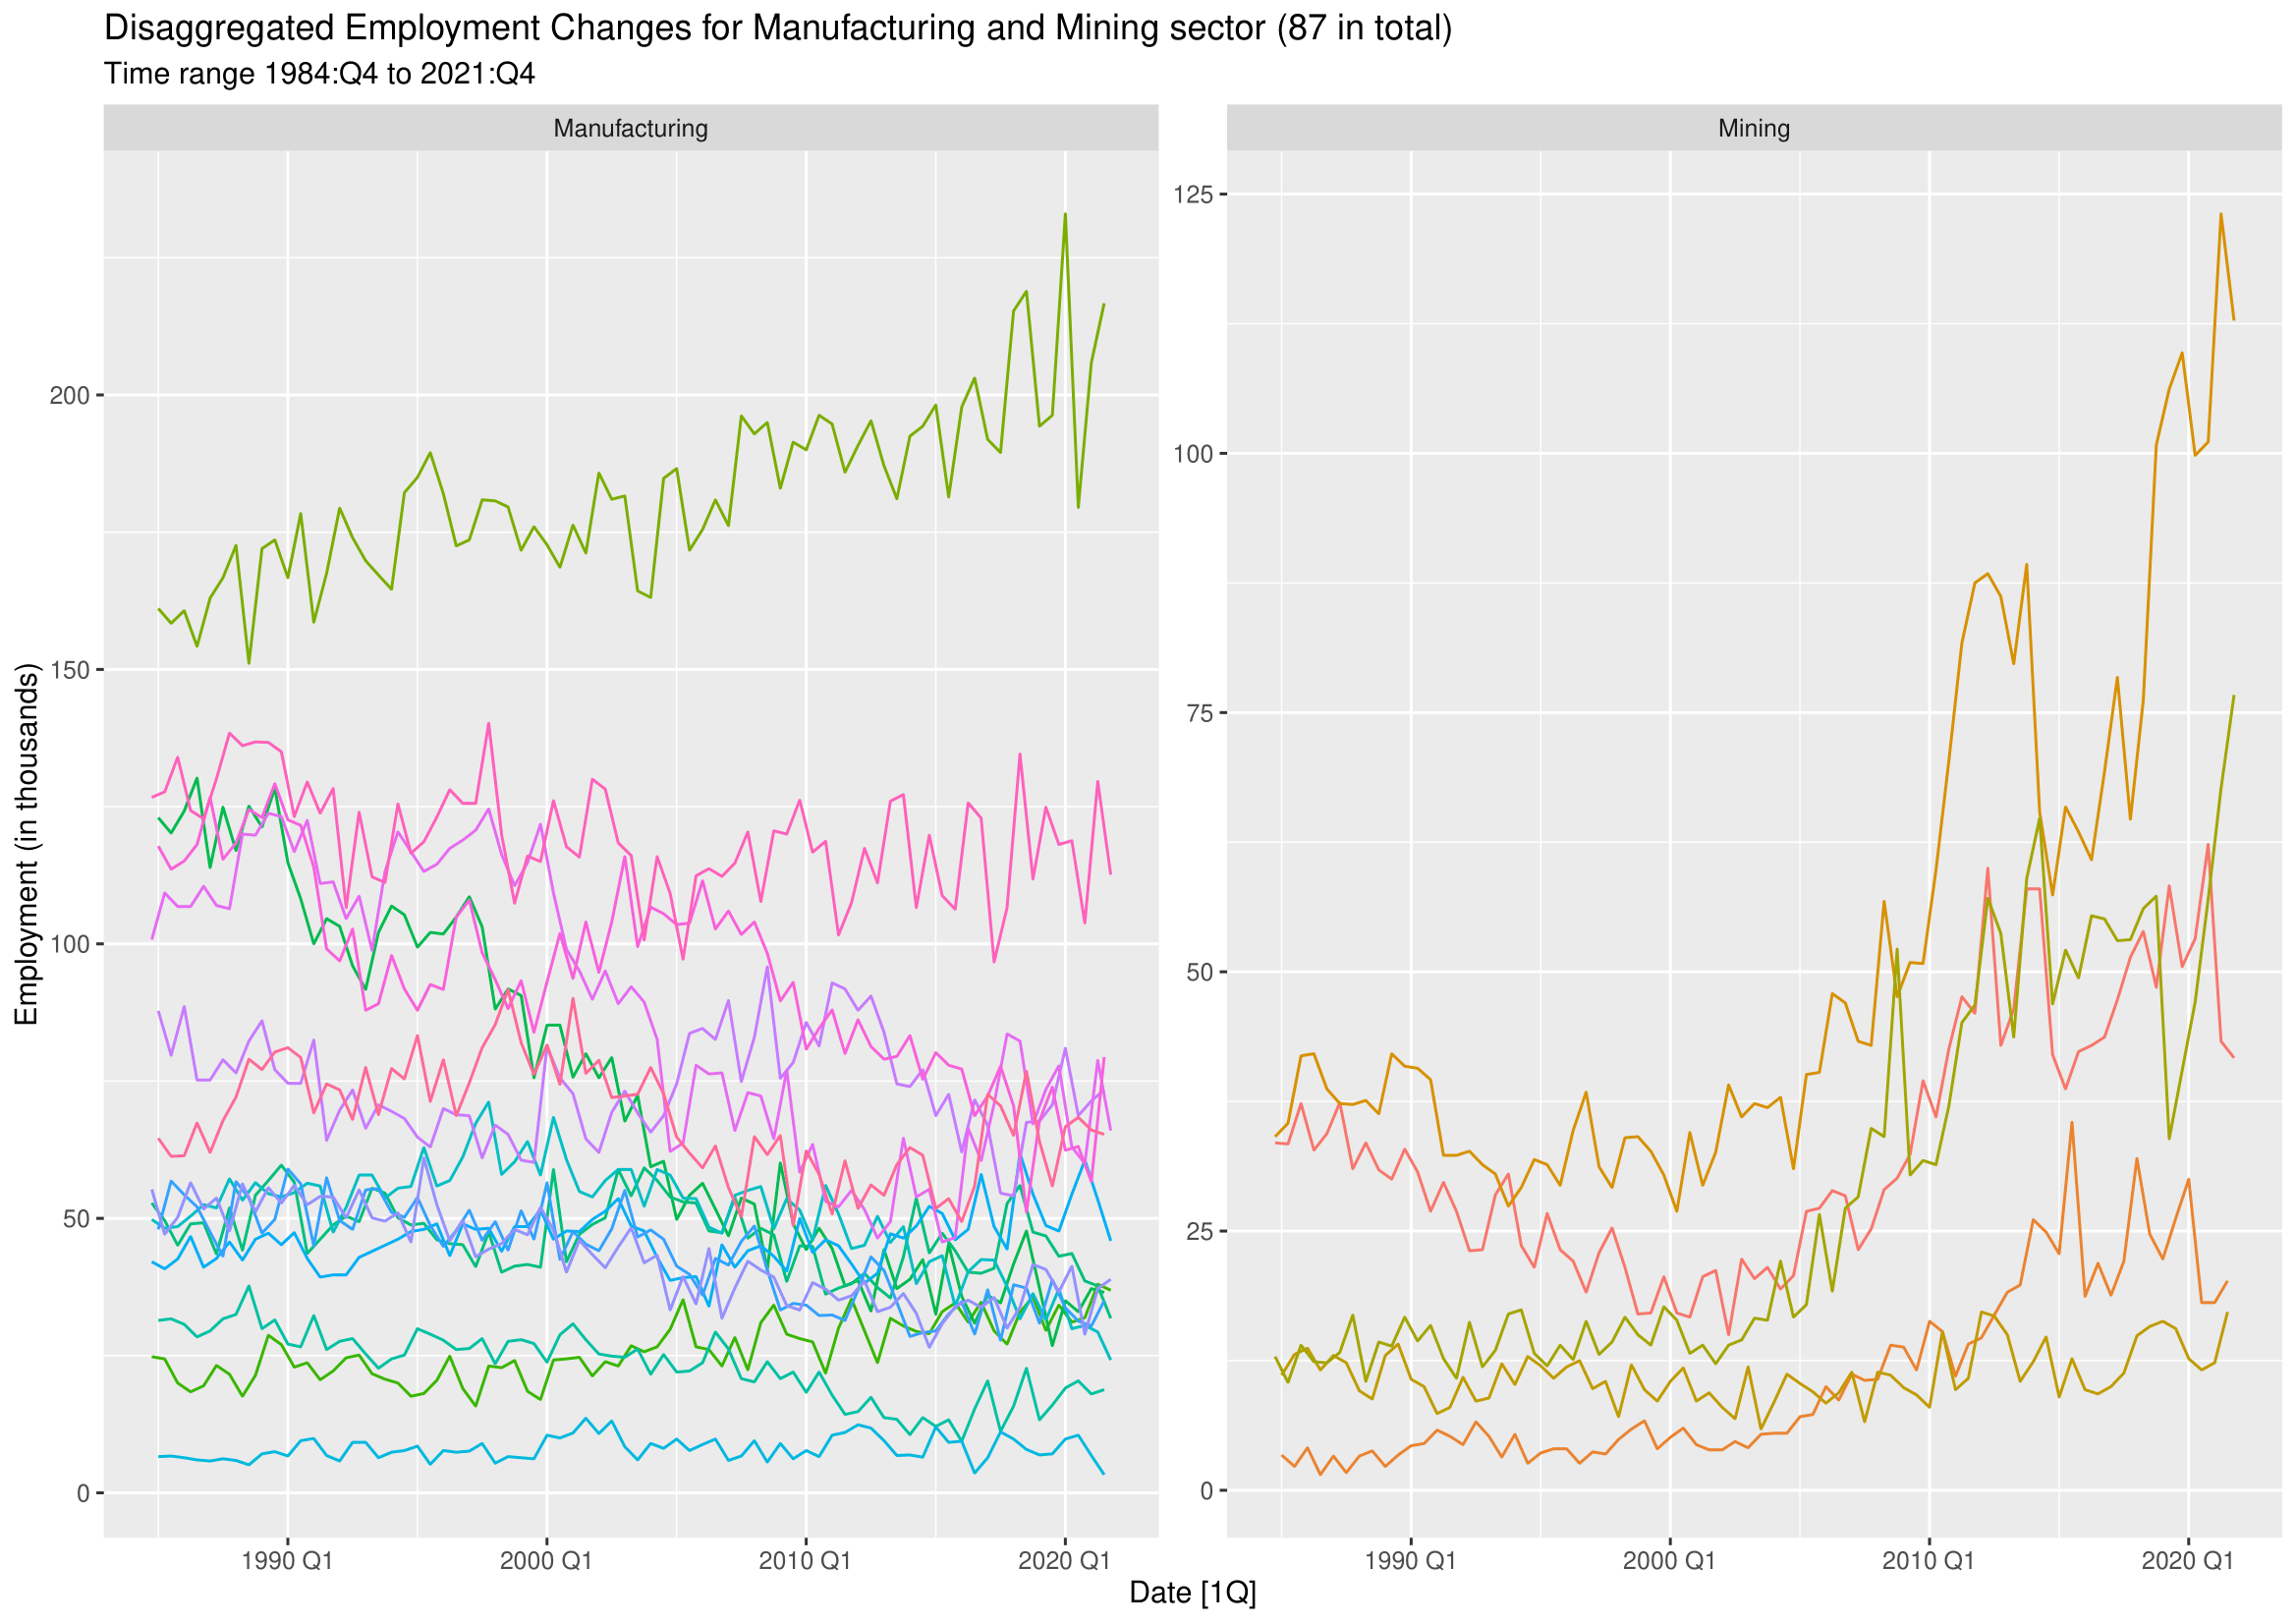
\includegraphics[scale=0.5]{agg_87}
\centering
\caption{Disaaggregate Employment(in thousands) of 87 two-digit subsectors in Manufacturing and Mining sector from 1984:Q4 to 2021:Q4}
\label{fig:a87}
\end{figure}

\begin{figure}[t]
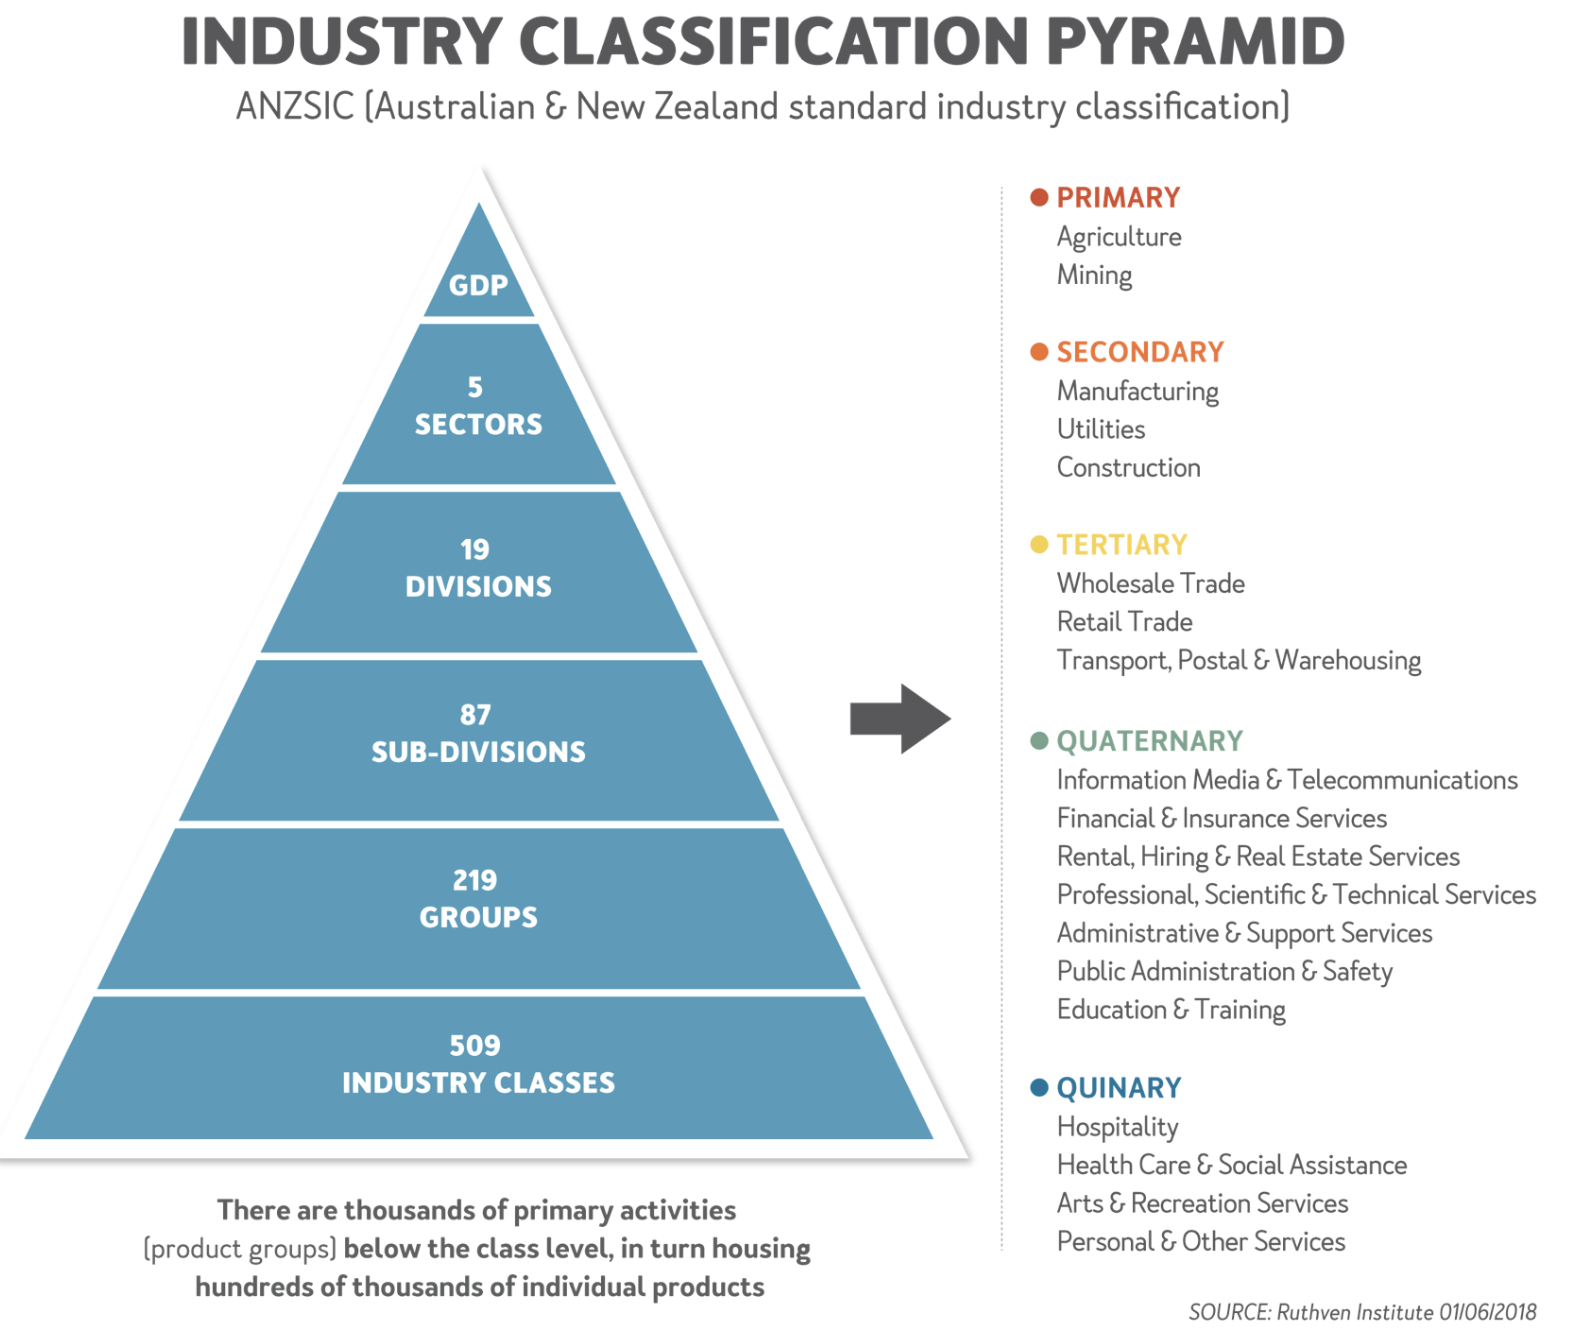
\includegraphics[scale=0.5]{ANZSIC}
\centering
\caption{Australian Industry Pamamid plot by (ANZSIC)}
\label{fig:anzsic}
\end{figure}

\printbibliography[heading=bibintoc]



\end{document}
